\begin{table*}[!tp]
    \centering
    \begin{tabular}{|l |c|}
        \hline        \rotatebox{90}{\hspace{3em}MIMIC-IV} 
        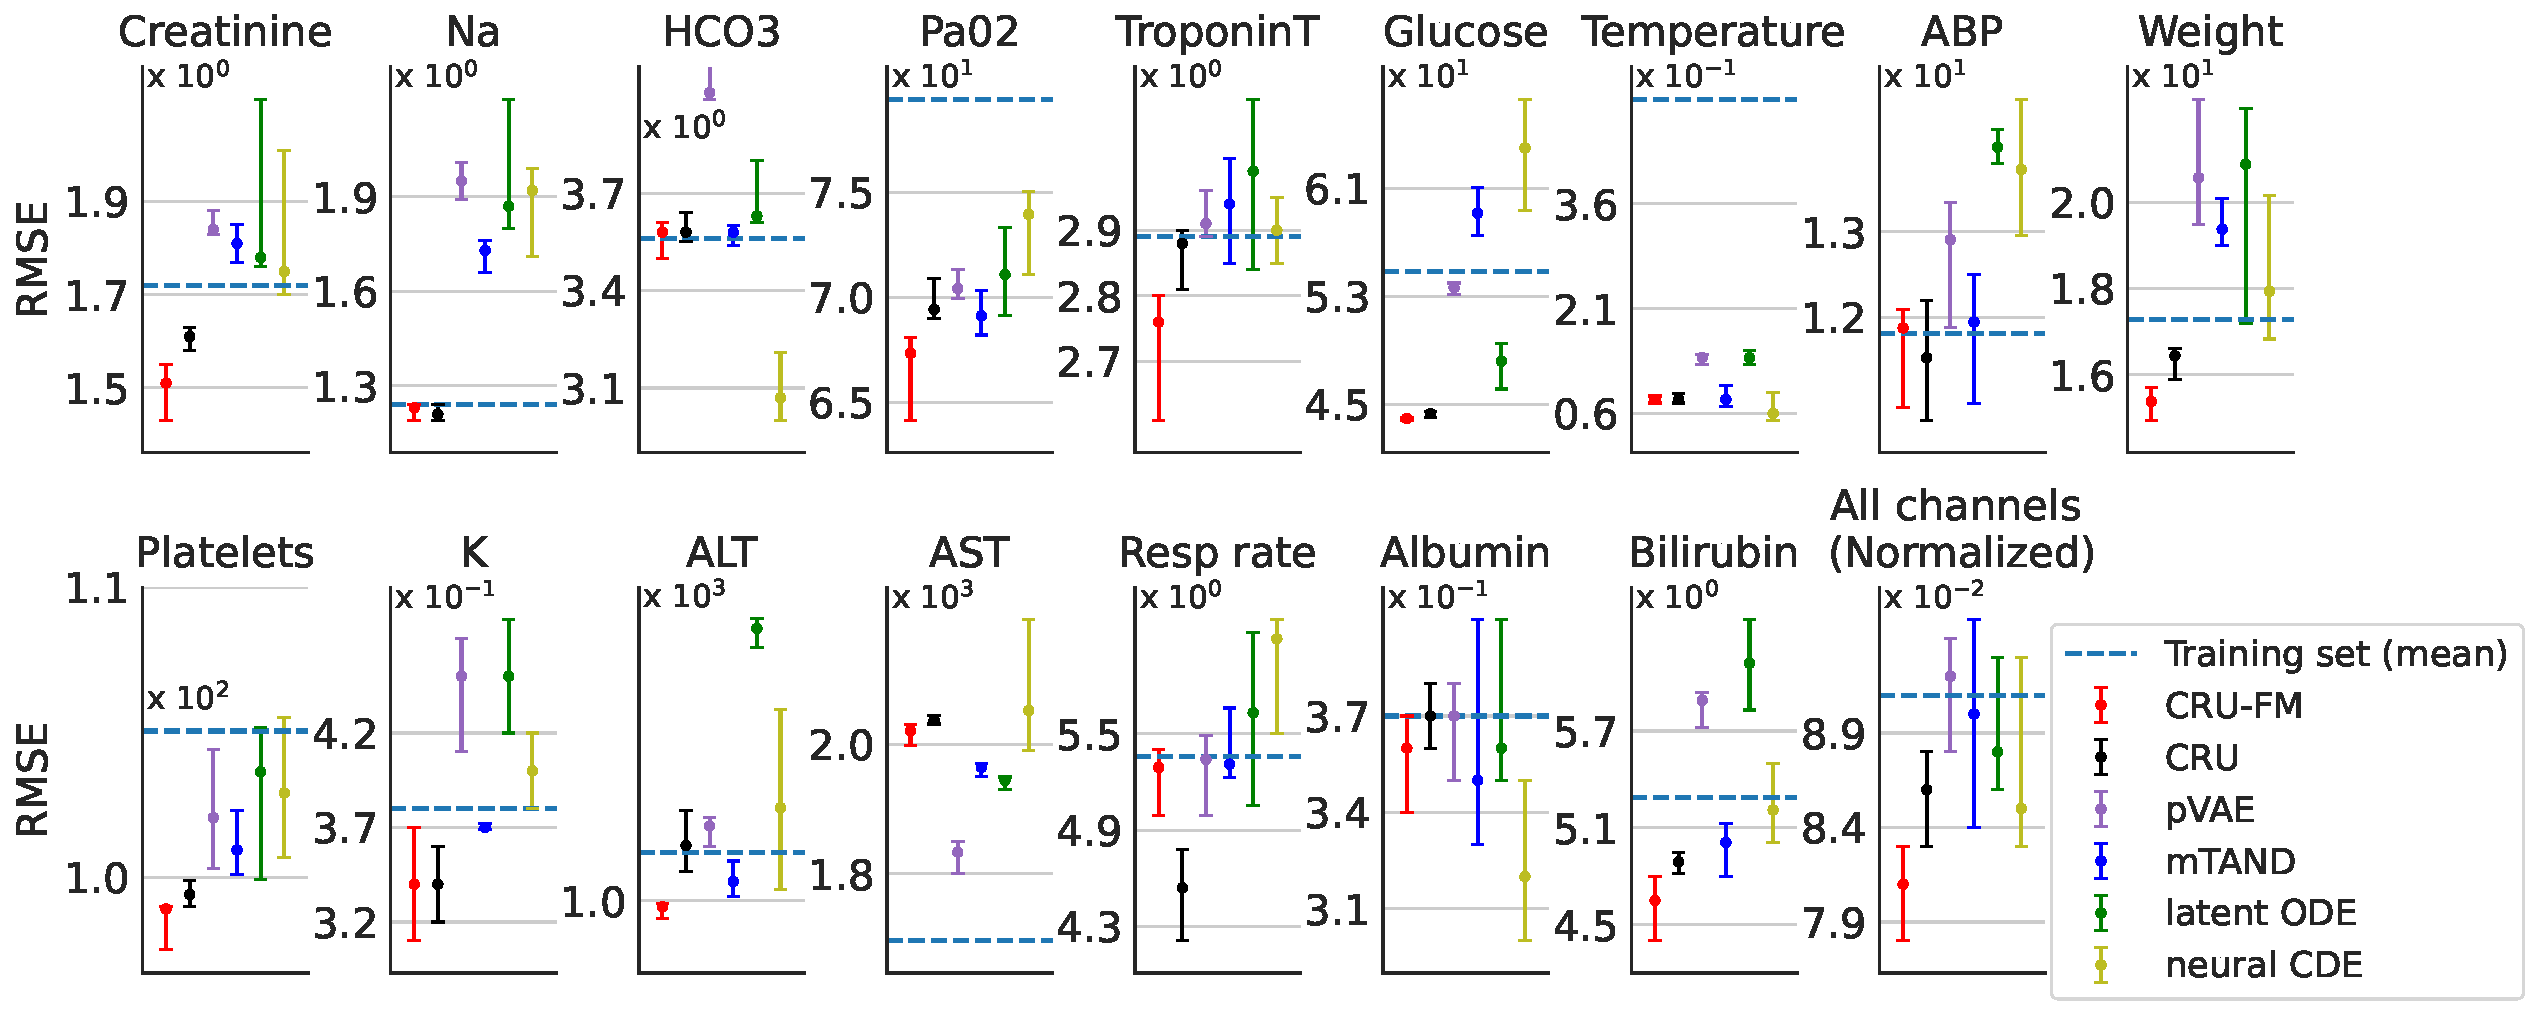
\includegraphics[width=0.95\textwidth]{content/chapters/irregular_time_series_data_driven_missingness/figures/mimic_evaluation.pdf} 
        \\~\\
        \hline
        \rotatebox{90}{\hspace{4em} Physionet} 
        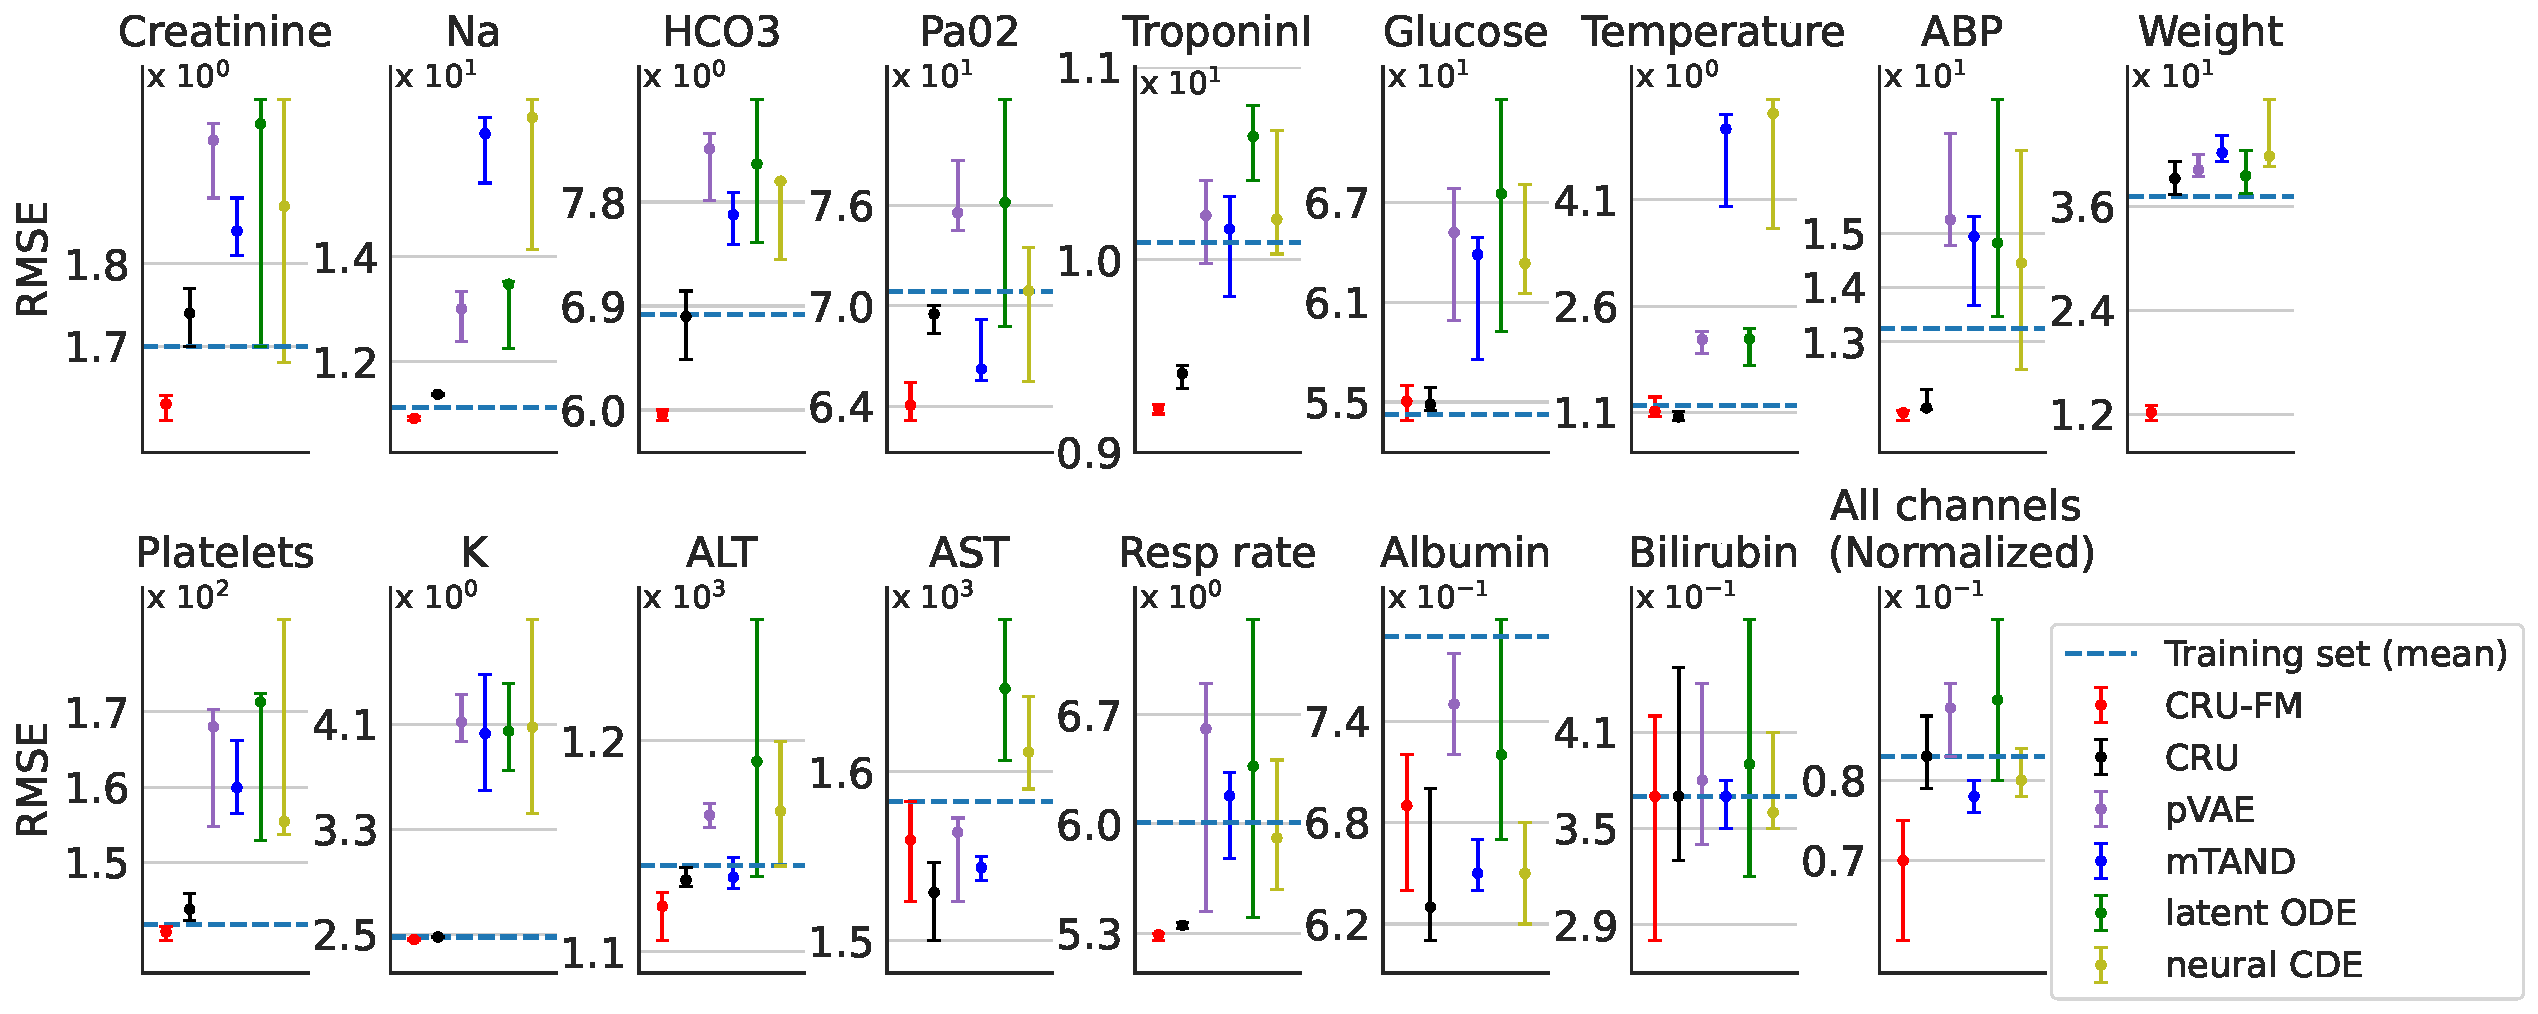
\includegraphics[width=0.95\textwidth]{content/chapters/irregular_time_series_data_driven_missingness/figures/physionet_evaluation.pdf} 
        \\~\\
        \hline
        \rotatebox{90}{\hspace{4em} eICU}
        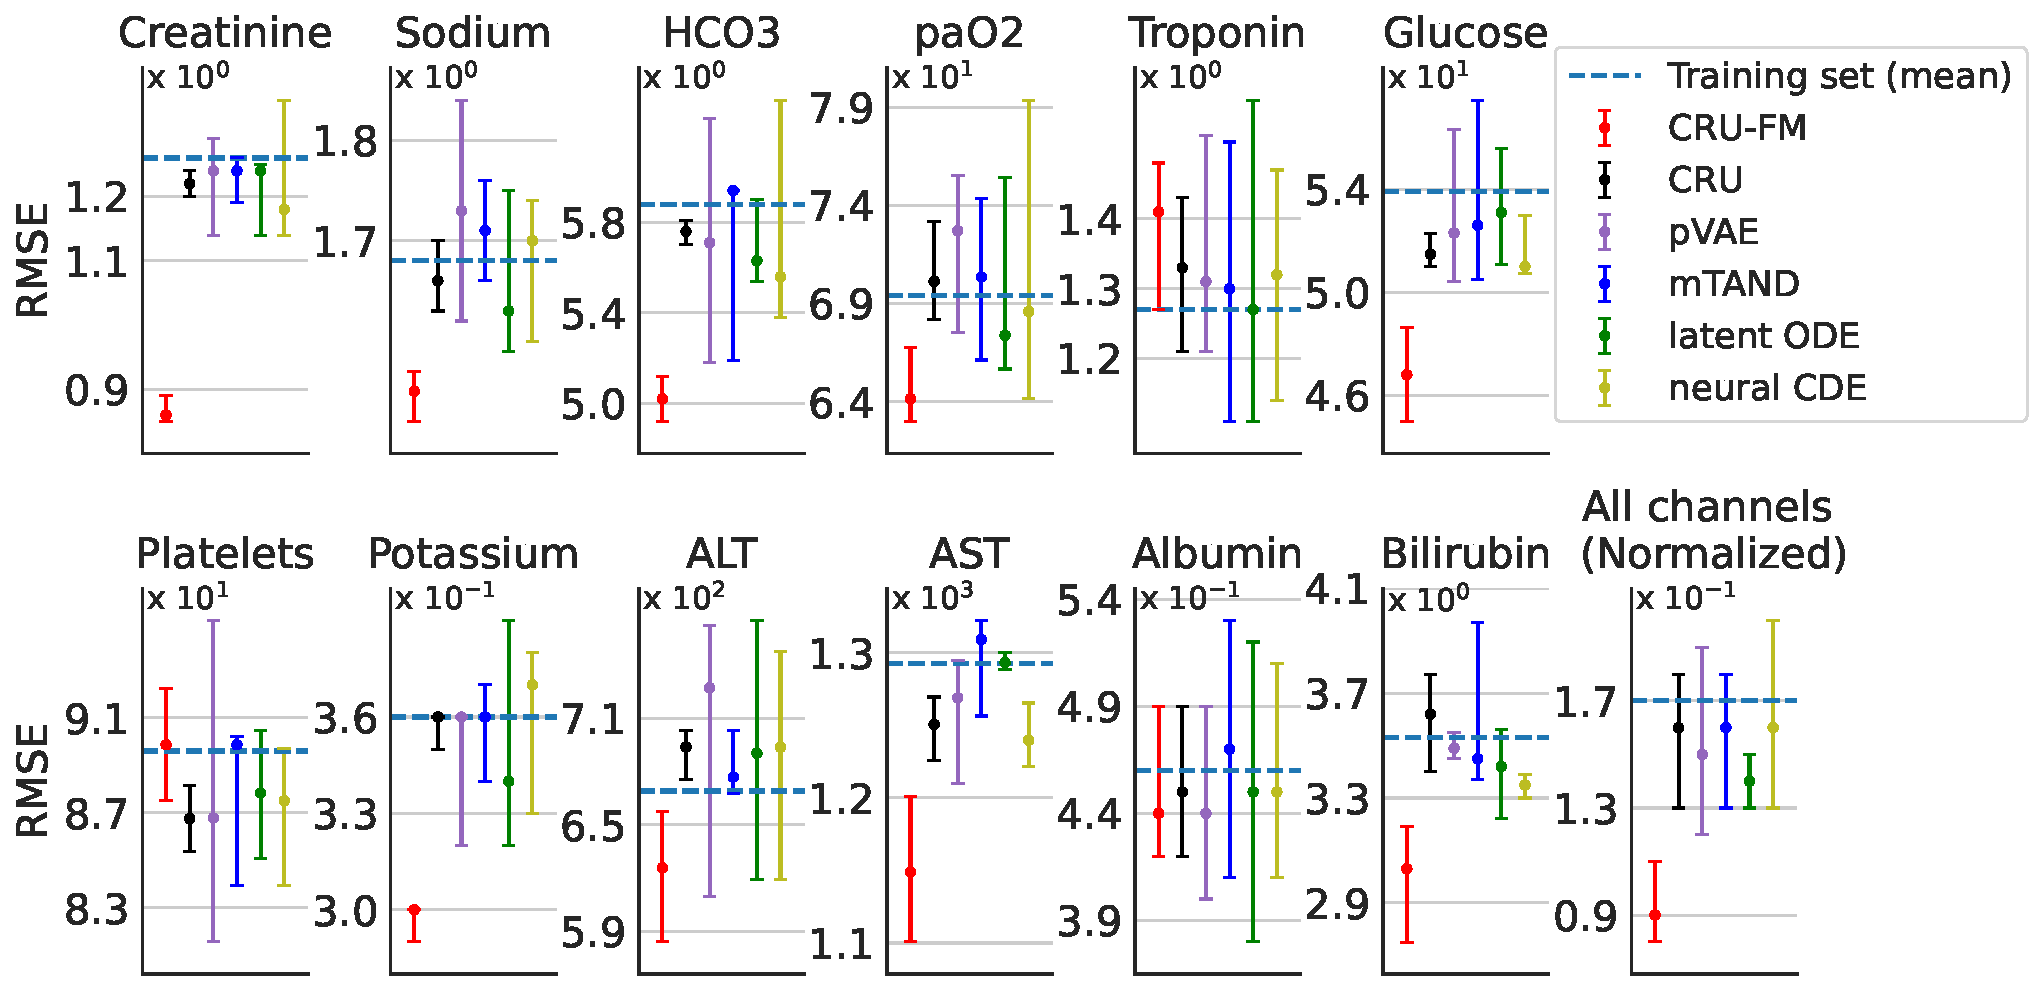
\includegraphics[width=0.95\textwidth]{content/chapters/irregular_time_series_data_driven_missingness/figures/eicu_evaluation.pdf}\\
        \hline
    \end{tabular}
    \caption[Extrapolation performance on extended list of channels on 3 EHR datasets comparing 5 baselines with our CRU-FM]{RMSE comparison of our CRU-FM with 5 baselines after training on the first 24 hours of data and extrapolating the next 24 hours of measurements on MIMIC-4, Physionet, and eICU. Confidence intervals represent the 5th and 95th percentiles from 100 bootstrapped samples from the test set. Our CRU-FM outperforms baselines in 8/16 channels in MIMIC-4, 11/16 channels on Physionet and 7/12 channels in eICU (RMSE confidence intervals are lower and do not overlap with baselines). The training set mean baseline is added to uncover a gap in existing studies \citep{shukla2021multitime, rubanova2019latent}, which overlooked a simple yet effective benchmark that, while showing decent RMSE performance, falls short in complex clinical decision-making settings.}
    \label{fig:all_channels_evaluation_extended}
\end{table*}